\section{Evaluation} \label{sec:eval}

We have evaluated our system on a 64-bit Dell server running Ubuntu
server 8.04 with kernel version 3.2.9. We used one Flash based SSD and
one SATA HDD. The SSD is an Intel SSDSA2CW300G3 2.5-inch with 300G
capacity. The SATA disk is a Maxtor 7L250S0 3.5-inch SATA HDD. Its
capacity is 250GB and its rotational speed is 7200 rpm.

\subsection{Benchmark Platform}

Firstly, we measured the two storage devices used in our benchmarks.
The results we got support our argument that Flash is good in random
I/O while HDD is not bad in sequential I/Os. We formated both devices
using Ext4. We remount devices before each benchmark to make sure that
all disk caches are dropped. The devices were measured using
Filebench~\cite{filebench-web}. Random read and write were measured
using Filebench built-in workloads \texttt{randomread} and
\texttt{randomwrite}; Sequential read and write were measured using
Filebench built-in workloads \texttt{singalstreamread} and
\texttt{singalstreamwrite}.

SSD vs SATA

\subsection{Wikipedia Image Workload}

We first show micro benchmark results on simple workloads of
sequential and random read and write of MRIS. To demonstrate the
benefits of multi-tier system, we experimented every workload on three
different setups. 

\begin{figure}[t]
\begin{centering}
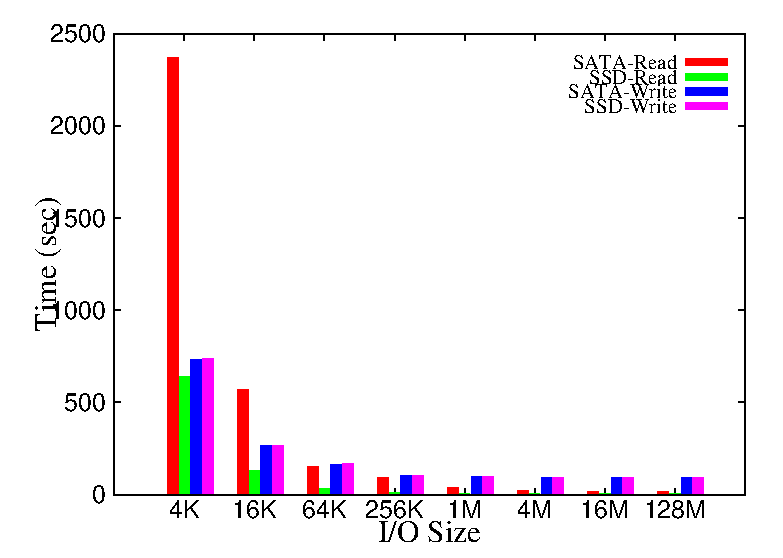
\epsfig{file=figures/raw_rand_speed.eps,width=1.00\linewidth}
\caption{I/O performance of the SSD and the SATA disk. }
\label{fig:ssd_vs_sata}
\end{centering}
\end{figure}

Before we evaluated the performance of out green target, we
benchmarked the performance of the two physical disks.  We measured
the time elapsed to read/write 1G of data randomly from the raw disks
of the SSD and the SATA using the Linux \texttt{dd} command. We set
the \texttt{direct} I/O flag in \texttt{dd} to make sure I/Os were
directly served by disks instead of cache in memory.  In the tests, we
also confined all I/Os to be within the first 1G of the two disks
because the capacities of the virtual devices we created in the rest
of the evaluation are 1G. The results are presented in Figure
\ref{fig:ssd_vs_sata}. The most salient trend in Figure
\ref{fig:ssd_vs_sata} is that I/O speed goes down quickly as I/O size
decreases. This is true for both disks and for both read and write. 

For read, the SSD is more than 4 times faster than the SATA disk on
average. Actually, the advantage of the SSD is less than 4$\times$
only when the I/O size is 4K.  One reason is that when I/O size is
small, the number of times we need to invoke \texttt{dd} to serve 1G
I/O is so large that the routines of executing commands, such as
command lookup, security check, and creating process, slow down the
test.  When the I/O size becomes as small as 4K, the number of
execution of the \texttt{dd} command becomes as large as 256K in order
to serve 1G I/O.  Particularly, when the I/O size is 256K, the SSD is
7 times faster than the SATA disk. 

For write, there is almost no differences between the SSD and the
SATA. For all I/O sizes, it took the same time to serve the same
amount of I/O. Moreover, writes of the SSD is significantly slower
than reads of the SSD.  However, write is not always slower than read
for the SATA disk. When the I/O size is small, e.g., 4K and 16K, write
of the SATA disk is much faster than read. This is because of the disk
cache within the SATA disk. Write can be served as long as the data
get written into the disk cache. However, for read, we have to read
from magnetic disks (unless it is within the small disk cache, which
is unlikely for random reads), which incurs movement of mechanic
components. This fact supports our design discussed in Section
\ref{sec:migrate}, which is we do not migrate extents on secondary
disks that are being written. 

\begin{figure}[t]
\begin{centering}
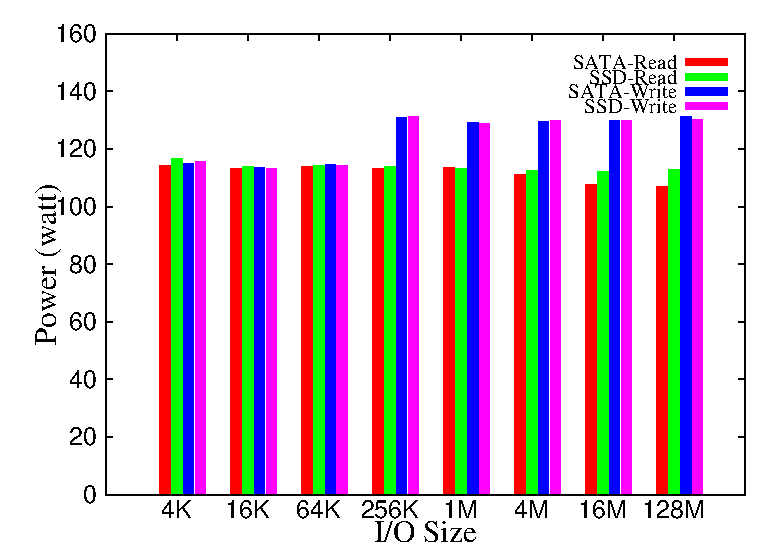
\epsfig{file=figures/raw_power.eps,width=1.00\linewidth}
\caption{Power of the SSD and the SATA disk.}
\label{fig:power}
\end{centering}
\end{figure}

\begin{figure}[t]
\begin{centering}
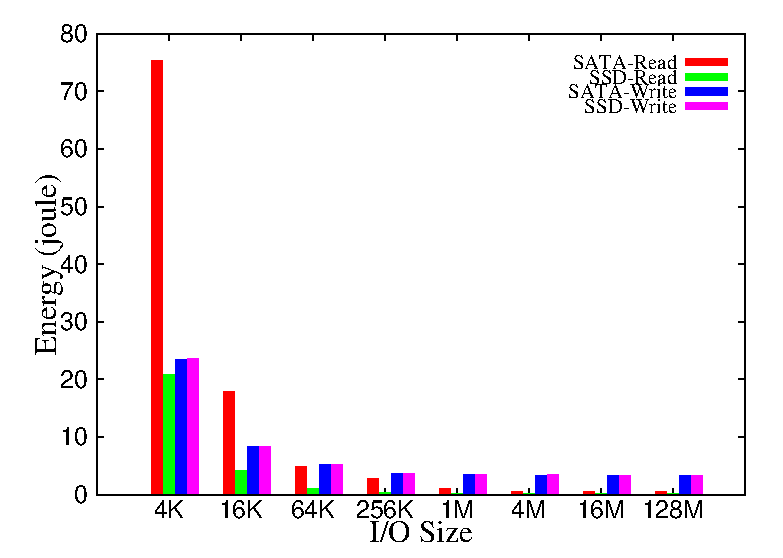
\epsfig{file=figures/raw_energy.eps,width=1.00\linewidth}
\caption{Energy of the SSD and the SATA disk.}
\label{fig:energy}
\end{centering}
\end{figure}

We have also collected the power and energy consumption data of the
tests. They are presented in Figure \ref{fig:power} and
\ref{fig:energy}. Because we did not spin the disks, the power of the
SSD and the SATA disk is close to each other. A remarkable trend in 
Figure \ref{fig:power} is that when I/O size is larger than 256K, the
power of writes is averagely 15 watt higher than smaller I/O sizes.
This is true for both the SSD and the SATA disk. Because the power is
stable, the energy is mainly affected by the time of the operations.
That is why Figure \ref{fig:energy} resembles Figure
\ref{fig:ssd_vs_sata}. 

\subsection{Facebook Workloads}

1. 17 of Ran R on three setups

2. RR workload of different ratios on hybrid.

To evaluate the green target, we created virtual devices using our
target, performed I/Os on the devices using \texttt{dd}, and compared
them with devices created by the linear target.  Both types of virtual
devices have the same configuration. They are 1G large, with the first
256M comes from the SSD and the rest comes from the SATA. The extent
size of the green device is 4K by default. The mapping table of the
linear and green virtual devices are presented in Figure
\ref{fig:dmtable} (a) and (b), wherein \texttt{/dev/sdd} is the SSD
and \texttt{/dev/sdc} is the SATA disk. 

To start with, we considered the best scenario first. It happens when
linear devices are accessing the SATA disk whereas green devices map
all I/Os onto the SSD.  In this experiment, we still measured the time
elapsed to read/write 1G of data from the green and linear device
using the Linux \texttt{dd} command.  We also confined the address
space covered by the I/Os to be within 256M so that the green disk can
map all of them on the SSD without migration.  We also make sure
offsets of all the I/Os are larger than 256M so that all I/Os are
served by the SATA for the linear device. However, in the case of the
green device, all I/Os are served by SSD thanks to the flexible
mapping mechanism.  

\subsection{Wikipedia Workloads}

We present the results in Figure \ref{fig:best}.  For read, the green
device is more than 3 times faster for all 7 different I/O sizes.
Particularly, when the I/O size is 64K and 256K, the speedup is more
than 7 and 5 times respectively. This suggests the green device can be
a good fit for workloads containing most I/Os of these sizes. However,
for write, the green device does not exhibit any advantage over the
linear device. This is the same as the comparison between writes of
the SSD and SATA disk. In fact, the whole Figure \ref{fig:best} and
Figure \ref{fig:ssd_vs_sata} are very close to each other. This is
exactly what we are expecting because, in the best scenario, the
linear device works using only the SATA disk, whereas the green device
works using only the SSD.

\begin{figure}[t]
\begin{centering}
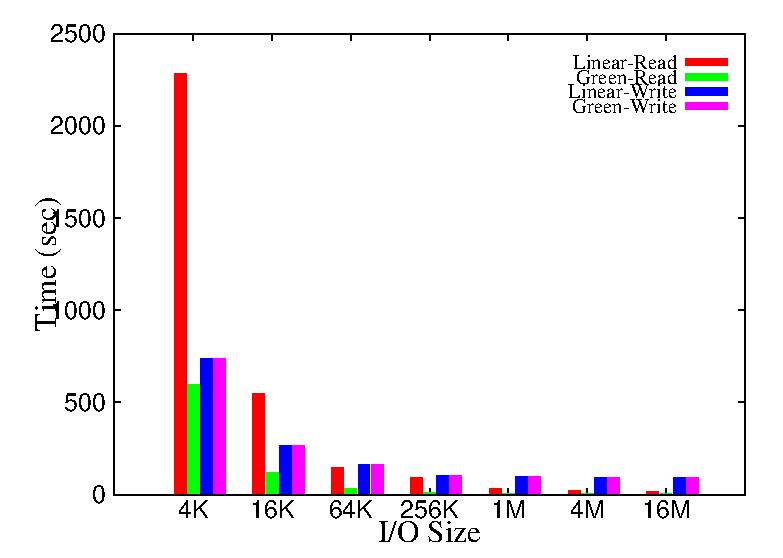
\epsfig{file=figures/best_speed.eps,width=1.00\linewidth}
\caption{Performance of green and linear devices in the best
scenario.}
\label{fig:best}
\end{centering}
\end{figure}

\subsection{The Middle Scenario}

\begin{figure}[t]
\begin{centering}
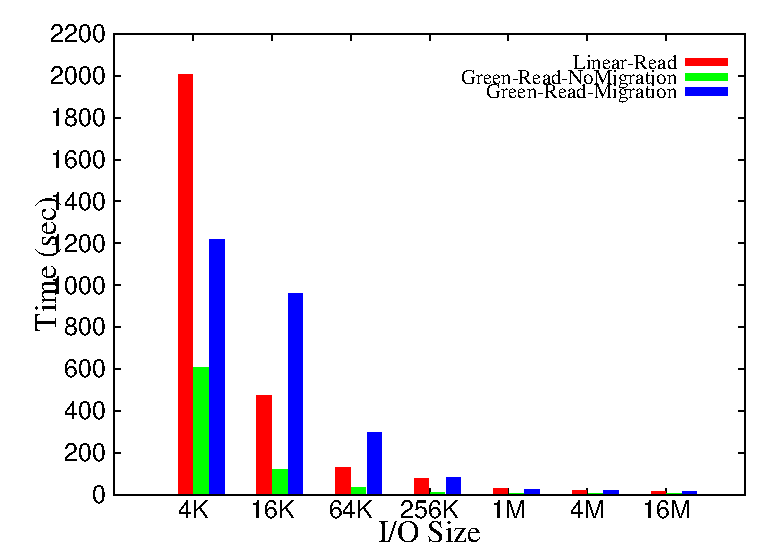
\epsfig{file=figures/even_read.eps,width=1.00\linewidth}
\caption{Performance of green (with and without migration) and linear
devices of read.}
\label{fig:evenread}
\end{centering}
\end{figure}

\begin{figure}[t]
\begin{centering}
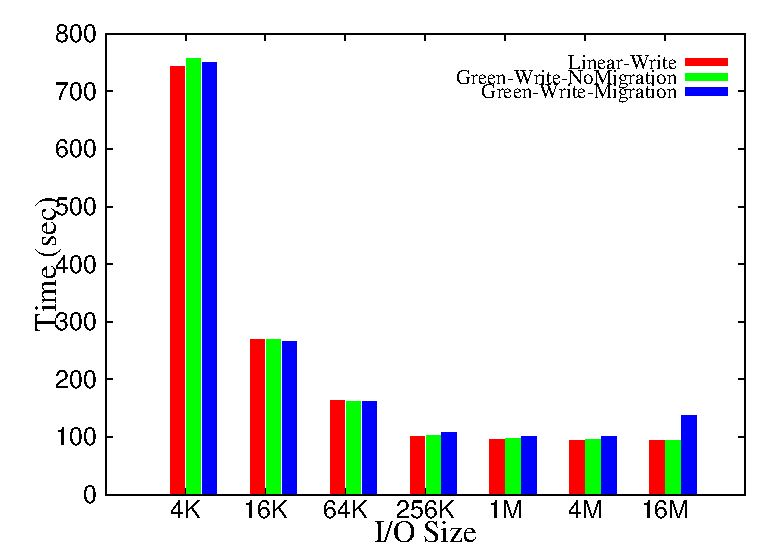
\epsfig{file=figures/even_write.eps,width=1.00\linewidth}
\caption{Performance of green (with and without migration) and linear
devices of write.}
\label{fig:evenwrite}
\end{centering}
\end{figure}

We considered a more realistic scenario, which we call \textit{middle}
scenario. In this scenario, we distributed I/Os evenly among whole
virtual devices, i.e., the whole virtual space backed by both the SSD
and SATA.  By evenly, we mean the number of I/Os served by the
underlying physical disks are proportional to their capacity.  In our
settings, offsets of one forth of the I/Os are less than 256M, while
the rest are larger than 256M.  We also confined the range covered by
all I/Os to be within 256M.  Therefore, it is still possible for our
green device to map all I/Os onto the SSD, whereas only 1/4 of the
I/Os are served by the SSD in the linear device case.  We compared the
linear device with two different configurations of the green device.
One configuration is we started with an empty green device; and the
other is we started with a half-full green device. The difference
between the two configurations is that data migration is needed to map
I/Os onto SSD for the latter. Therefore, the three cases we compared
here are linear, \textit{green-migration}, and
\textit{green-no-migration}.

The results of reads of the three cases are shown in Figure
\ref{fig:evenread}. Not surprisingly, the best case is
green-no-migration. It is 3 times faster than the linear case for all
I/O sizes. The performance of the green-migration case is not between
the green case and the green-no-migration. When the I/O size is large,
i.e., larger than 64K in Figure \ref{fig:evenread}, the performance of
green-migration is almost the same as linear. It seems the green
device behaves with no difference to the linear device. This is true.
Because when I/O size is large, I/O mapping requests come to the green
device in burst. However, extent migration is a slow asynchronous
operation and I/Os involved in migration can be served only after
related migrations are finished. To reduce latency, as discussed in
Section \ref{sec:implementation}, we set a limit of the maximum number
of active migrations. Therefore, very few migrations are performed in
this case, which makes the green device just like a linear device.  As
the I/O size goes down, more migrations are performed. Because
migration is expensive and can benefit performance only when migrated
extents are heavily used. When the I/O size is 16K and 64K,
significant amount of migrations are scheduled that the I/O
performance is negatively affected. But the I/O process is not long
enough that the migrated extents do not get too much chance to be
accessed again. When the I/O size becomes small enough, namely 4K
here, migrated extents benefit more subsequential I/Os and offset the
cost of migrations. In Figure \ref{fig:evenread}, green-migration
demonstrates significant advantage over linear.

Moreover, the performance of green-no-migration is the same as the
performance of the green device in Figure \ref{fig:best}. This is
because both of them are serving all I/Os using SSD. The performance
of linear in Figure \ref{fig:evenread} is slight better than the
linear device in Figure \ref{fig:best}. This is because the former
serves 1/4 of the I/Os using the SSD whereas the latter serves all the
I/Os using the SATA disk.

The results of writes are shown in Figure \ref{fig:evenread}. Just
like write performance in previous scenario, there is no big
difference among the three cases. This, again, supports our design
strategy discussed in Section \ref{sec:migrate}.

\subsection{The Worst Scenario}

The worst scenario of the green device happens when it performs a lot
of migrations, but none of the migrated extents are accessed again
until they become LRU extents and get evicted. This is the case when
we scan the whole disk. Figure \ref{fig:worst} presents the elapsed
time to scan the green and the linear disk once with different I/O
sizes. Both the green and the linear disk are 1G large. The first 256M
comes from the SSD and the rest comes from the SATA disk.

For read, the green device is significant slower than the linear
device. This is reasonable because many migrations are performed but
wasted. The gap between the green and the linear diminishes as I/O
sizes become larger. Because large I/O sizes issue I/Os in short burst,
less migrations are allowed in short periods. Actually, the linear
device finishes the scan using the same amount of time for all I/O
sizes except 4K. This is because the I/Os are sequential as we scan
the disk. The I/O sizes do not make too much difference in this case.
The long time of the 4K I/O size is most likely because of the cost of
issue the \texttt{dd} commands. 

For write, the green device is also slower than the linear device. The
elapsed time of the green device goes down as the I/O size increase,
whereas the time of the linear device does not change. The writes of
the linear device is stable also because I/Os are sequential. The time
of the 4K I/O size does not stand out because writes are slower than
reads. It is the I/O latency, not the command executions, that
dominates the cost. 

Our system presents up to 5.3$\times$ speedup over the single-tier
store using HDD, or 62\% of the single-tier store using only Flash .
Particularly, for a workload emulating Facebook's photo requests, we
improve the throughput by XXX using only a small Flash of 5.9\% of the
total storage capacity.

\begin{figure}[t]
\begin{centering}
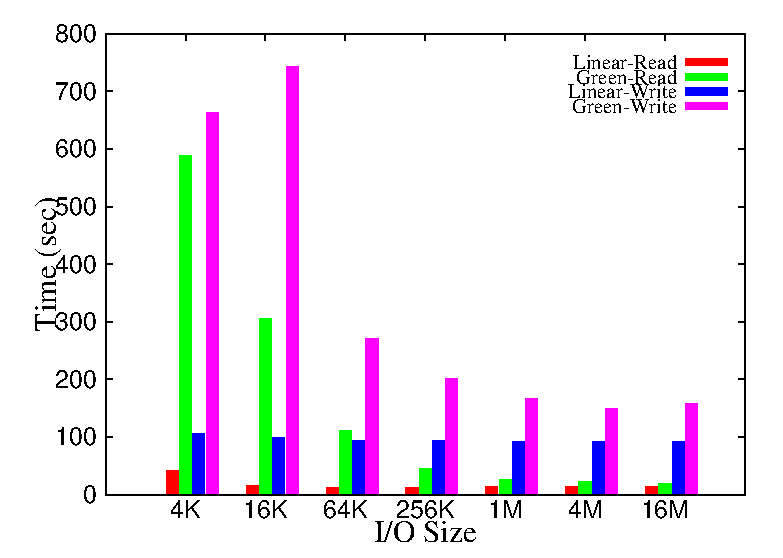
\epsfig{file=figures/worst.eps,width=1.00\linewidth}
\caption{Performance of green and linear in the worst scenario. }
\label{fig:worst}
\end{centering}
\end{figure}


%\subsection{Effect of Data Migration}

%Data migration is expensive. It includes two disk I/Os and is
%performed asynchronously. However, it is beneficial if the migrated
%data is heavily used so that the advantage of the SSD can offset the
%penalty of data migration. We studied the effect of data migration in
%this section. We initilized the green device as half-full. Because the
%green device always uses the SSD up first, the SSD becomes full and
%migrations are performed when data out of the SSD is accessed. We
%confined I/Os to cover a region less than 256M, which is the size of
%the SSD in our green device. We issued I/Os to the small region
%multiple rounds until 4G data is read. We measured the elapsed time
%for each round and compare it with the linear device.

%%%%%%%%%%%%%%%%%%%%%%%%%%%%%%%%%%%%%%%%%%%%%%%%%%%%%%%%%%%%%%%%%%%%%%%%%%%%%%
%% For Emacs:
% Local variables:
% fill-column: 70
% End:
%%%%%%%%%%%%%%%%%%%%%%%%%%%%%%%%%%%%%%%%%%%%%%%%%%%%%%%%%%%%%%%%%%%%%%%%%%%%%%
%% For Vim:
% vim:textwidth=70
%%%%%%%%%%%%%%%%%%%%%%%%%%%%%%%%%%%%%%%%%%%%%%%%%%%%%%%%%%%%%%%%%%%%%%%%%%%%%%
% LocalWords:  
